\documentclass[10pt,a4paper]{article}
\usepackage[utf8]{inputenc}
\usepackage[T1]{fontenc}
\usepackage{lmodern}
\usepackage[english]{babel}
\usepackage[margin=2.0cm]{geometry}
\usepackage{amsmath,amssymb,mathtools,bm}
\usepackage{booktabs,array,tabularx,longtable}
\newcolumntype{L}[1]{>{\raggedright\arraybackslash}p{#1}}
\newcolumntype{Y}{>{\raggedright\arraybackslash}X}
\usepackage{graphicx}
\usepackage{float}
\usepackage[font=small]{caption}
\usepackage{xcolor}
\usepackage{tikz}
\usetikzlibrary{arrows.meta,positioning,calc,fit,backgrounds}
\usepackage[hidelinks]{hyperref}
\usepackage{url}
\makeatletter\g@addto@macro{\UrlBreaks}{\do\_\do/}\makeatother
\numberwithin{equation}{section}
\setlength{\emergencystretch}{3em}
\newcommand{\note}[1]{\begin{center}\fcolorbox{red!70!black}{red!5}{\parbox{0.94\linewidth}{\small\textbf{Note.} #1}}\end{center}}
\newcommand{\psiMax}{5.74}
\newcommand{\thMin}{2.60}
\newcommand{\thMax}{3.18}
\newcommand{\dpsiMax}{1.27}
\newcommand{\dthMax}{0.059}
\newcommand{\period}{31.4}
\newcommand{\followAz}{182}
\newcommand{\ErmsCur}{26.6}
\newcommand{\ErmsDob}{2.72}
\newcommand{\ErmsIdeal}{2.70}
\newcommand{\EmaxCur}{131}
\newcommand{\EmaxDob}{8.0}
\newcommand{\EratioRms}{10}
\newcommand{\EratioMax}{16}
\newcommand{\JoneCur}{99}
\newcommand{\JoneDob}{9.7}
\newcommand{\JoneIdeal}{5.0}
\newcommand{\JoneRatio}{10}
\newcommand{\JtenCur}{1.88}
\newcommand{\JtenDob}{2.61}
\newcommand{\JtenIdeal}{0.011}
\newcommand{\JhunCur}{$4.6\cdot10^{-4}$}
\newcommand{\JhunDob}{0.14}
\newcommand{\BandOneTenCur}{99}
\newcommand{\BandOneTenDob}{9.3}
\newcommand{\BandTenHunCur}{1.88}
\newcommand{\BandTenHunDob}{2.61}
\newcommand{\NoiseJone}{8.2}
\newcommand{\IffNoise}{1.3}
\newcommand{\IffAz}{2.86}
\newcommand{\IffAzIdeal}{2.55}
\newcommand{\ErmsNoFFCur}{124}
\newcommand{\ErmsNoFFDob}{118}
\newcommand{\ErmsZoh}{2.90}
\newcommand{\ErmsCurZoh}{26.7}
\newcommand{\gyroNoise}{0.069}
\newcommand{\twist}{2.75}
\newcommand{\encAzDob}{0.54}
\newcommand{\JsweepFive}{42.5}
\newcommand{\JsweepTen}{18.4}
\newcommand{\JsweepTwenty}{9.7}
\newcommand{\JsweepForty}{10.3}
\newcommand{\noiseFloor}{5.9}
\newcommand{\noiseFloorTen}{1.3}
\newcommand{\arwSI}{3.78}
\newcommand{\tauRmsCurAz}{0.65}
\newcommand{\tauPkCurAz}{1.84}
\newcommand{\tauLoCurAz}{0.65}
\newcommand{\tauHiCurAz}{0.01}
\newcommand{\tauRmsIdealAz}{0.63}
\newcommand{\tauPkIdealAz}{1.84}
\newcommand{\tauLoIdealAz}{0.63}
\newcommand{\tauHiIdealAz}{0.00}
\newcommand{\tauRmsDobAz}{0.71}
\newcommand{\tauPkDobAz}{2.69}
\newcommand{\tauLoDobAz}{0.63}
\newcommand{\tauHiDobAz}{0.33}
\newcommand{\fricCurAz}{0.45}
\newcommand{\fricIdealAz}{0.46}
\newcommand{\fricDobAz}{0.46}
\newcommand{\cableAz}{-0.04}
\newcommand{\tauInertiaAz}{9.1}
\newcommand{\tauRmsCurEl}{0.46}
\newcommand{\tauPkCurEl}{0.62}
\newcommand{\tauLoCurEl}{0.46}
\newcommand{\tauHiCurEl}{0.00}
\newcommand{\tauRmsIdealEl}{0.46}
\newcommand{\tauPkIdealEl}{0.62}
\newcommand{\tauLoIdealEl}{0.46}
\newcommand{\tauHiIdealEl}{0.00}
\newcommand{\tauRmsDobEl}{0.37}
\newcommand{\tauPkDobEl}{0.97}
\newcommand{\tauLoDobEl}{0.36}
\newcommand{\tauHiDobEl}{0.11}
\newcommand{\fricCurEl}{0.43}
\newcommand{\fricIdealEl}{0.43}
\newcommand{\fricDobEl}{0.30}
\newcommand{\cableEl}{-0.15}
\newcommand{\tauInertiaEl}{0.2}
\newcommand{\tCont}{2.18}
\newcommand{\tPeak}{6.74}
\newcommand{\revAz}{8.4}
\newcommand{\revEl}{15.7}
\newcommand{\floorAz}{76.4}
\newcommand{\kIAz}{4329}
\newcommand{\ktkAz}{0.249}
\newcommand{\lowCurAz}{583}
\newcommand{\highHundAz}{1.17}
\newcommand{\peakFAz}{0.6}
\newcommand{\peakGAz}{1353}
\newcommand{\oneCurAz}{1268}
\newcommand{\oneDobAz}{124}
\newcommand{\floorEl}{0.0}
\newcommand{\kIEl}{6599}
\newcommand{\ktkEl}{0.276}
\newcommand{\lowCurEl}{345}
\newcommand{\highHundEl}{2.81}
\newcommand{\peakFEl}{2.8}
\newcommand{\peakGEl}{5704}
\newcommand{\oneCurEl}{2560}
\newcommand{\oneDobEl}{153}

\tikzset{
  blk/.style={draw, rectangle, minimum height=8mm, minimum width=9mm, align=center, font=\scriptsize, fill=white},
  sum/.style={draw, circle, inner sep=0pt, minimum size=4.5mm, font=\scriptsize},
  sig/.style={-{Latex[length=1.8mm]}, thick},
  lab/.style={font=\scriptsize},
  grp/.style={draw, dashed, rounded corners, inner sep=2.5mm},
}

\title{Disturbance rejection with a gyro-based reduced-order observer\\ for the LUCY pointer: implementation and results on a tracking task}
\author{Generated by \texttt{build\_dob\_report.py}\\ \small\texttt{sim/gimbal\_multidof/closedLoopModel/report\_dob}}
\date{\today}
\begin{document}
\maketitle

\paragraph{Purpose.} This report describes, step by step, how the disturbance observer proposed by Hilkert and Pautler~\cite{hilkert2011} was added to the time-domain model of the LUCY pointer, and how it was compared with the current control structure on the tracking task of Attorrese~\cite{attorrese2026}: a drone flying a circle of radius 10\,m at 5\,m of height, 100\,m away, at 0.2\,rad/s. The comparison is done twice:
\begin{itemize}
\item with a continuous loop and an ideal gyro, to see what the structure can do;
\item with the constraints of the real signals: drives on an EtherCAT network with process data every 1\,ms, and a MEMS gyro (Analog Devices ADIS16507~\cite{adis16507}) read over SPI, with its second-order dynamics and the noise of its Allan deviation.
\end{itemize}
The focus is on the pointing error and on the jitter of the line of sight, current structure against the observer with the noisy gyro.

\paragraph{Main results} (EtherCAT and ADIS16507, velocity feedforward of the drives on, one orbit; line of sight of the telescope).
\begin{itemize}
\item \textbf{Pointing error:} \ErmsCur\ mdeg rms (\EmaxCur\ mdeg max) with the current structure, \ErmsDob\ mdeg rms (\EmaxDob\ mdeg max) with the observer: \EratioRms\ times lower in rms, \EratioMax\ times lower at the peak.
\item \textbf{Jitter above 1\,Hz:} \JoneCur\ $\mu$rad with the current structure, \JoneDob\ $\mu$rad with the observer and the noisy gyro (\JoneIdeal\ $\mu$rad with an ideal one): \JoneRatio\ times lower.
\item \textbf{Jitter above 10\,Hz:} slightly higher with the observer (\JtenDob\ against \JtenCur\ $\mu$rad), and much higher above 100\,Hz (\JhunDob\ $\mu$rad against \JhunCur\ $\mu$rad, negligible in absolute terms). This is the gyro noise, differentiated by the observer and fed to the motor (Hilkert's noise-coupling trade-off~\cite[eq.~9]{hilkert2011}).
\item \textbf{Without the velocity feedforward} (as in the tests of October) the pointing error is the following error of the position loop, about \ErmsNoFFCur\ mdeg rms, and the observer cannot reduce it: by construction it does not change the response to the command.
\item \textbf{Required torque:} with an ideal gyro the observer asks for the same torque as the current structure (rms \tauRmsCurAz\ and \tauRmsIdealAz\,N\,m in azimuth), only earlier at the velocity reversals. With the ADIS16507 the azimuth torque carries \tauHiDobAz\,N\,m rms of noise above 10\,Hz, with a peak of \tauPkDobAz\,N\,m (40\,\% of the peak torque of the motor).
\item EtherCAT at 1\,ms changes the pointing error by hundredths of a millidegree; the observer must pass through a notch on the first structural mode of the elevation to be stable above 7\,Hz.
\end{itemize}

\tableofcontents

%% ===================================================================================================
\section{Task and model}\label{sec:task}
\subsection{Tracking task}
The reference is the one of Attorrese~\cite[sec.~6.2]{attorrese2026} (Figure~\ref{fig:reference}): pointer at the origin, drone on a horizontal circle of radius $R=10$\,m at height $h=5$\,m, centred at $(100,0)$\,m, angular rate $\omega=0.2$\,rad/s (period \period\,s). With the drone at $(x,y,h)$, the pointing angles and rates are
\begin{equation}
\psi=\operatorname{atan2}(y,x),\quad \theta=\operatorname{atan2}\bigl(h,\rho\bigr),\quad \rho=\sqrt{x^2+y^2},\quad
\dot\psi=\frac{x\dot y-y\dot x}{\rho^2},\quad \dot\theta=-\frac{h\,\dot\rho}{\rho^2+h^2}.
\end{equation}
\begin{itemize}
\item The azimuth swings $\pm\psiMax^\circ$ at up to \dpsiMax\,deg/s, with two reversals per orbit.
\item The elevation moves between \thMin\ and \thMax$^\circ$ at up to \dthMax\,deg/s: always in the low-speed range of the friction.
\end{itemize}
The pointer starts at rest on the reference; the metrics use one orbit after 5\,s of settling.
\begin{figure}[H]\centering
\includegraphics[width=\linewidth]{figures/reference.pdf}
\caption{Reference: top view of the circle [m], pointing angles [deg] and rates [deg/s] against time [s].}\label{fig:reference}
\end{figure}

\subsection{Model of the pointer}
The time-domain model is the one of the earlier reports: the 8-DOF lumped plant H6 (plant fitted on the October frequency responses), the TBM7646 motors and the AKD2G drives, with
\begin{itemize}
\item the effective gains of the drives identified on the step tests (iteration I5);
\item the bearing friction (Dahl element with a Stribeck level), the cable spring $K_c(\theta-\theta_0)$ and the torque scale $\kappa_i$ identified on the V2 doublets.
\end{itemize}
\begin{table}[H]\centering\scriptsize\setlength{\tabcolsep}{3pt}
\caption{Parameters of the model per axis: drive gains (I5), torque scale, friction (Coulomb level, break-away level, Stribeck speed, pre-sliding stiffness), cable spring (V2), and the rigid inertia $J'=\mathbf r^T\mathbf M\mathbf r$ used by the observer.}\label{tab:model}
\begin{tabular}{lrrrrrrrrrrr}\toprule
& $K_{pp}$ & $K_{pv}$ & $K_{iv}$ & $\kappa_i$ & $T_c$ & $T_s$ & $v_s$ & $\sigma_0$ & $K_c$ & $\theta_0$ & $J'$ \\
axis & [1/s] & [A\,s/rad] & [Hz] & [--] & [N\,m] & [N\,m] & [deg/s] & [N\,m/rad] & [N\,m/rad] & [deg] & [kg\,m$^2$] \\ \midrule
azimuth & 6.98 & 379 & 0.26 & 0.96 & 0.23 & 1.84 & 0.33 & 4513 & 0.93 & -2.68 & 2.162 \\
elevation & 6.78 & 54 & 2.88 & 1.07 & 0.41 & 0.46 & 0.86 & 1703 & 1.66 & -2.16 & 0.900
\\ \bottomrule
\end{tabular}\end{table}

%% ===================================================================================================
\section{Control architectures}\label{sec:arch}
\subsection{Current structure}
In the terms of Hilkert's review of inertially stabilised platforms~\cite{hilkert2008}, LUCY today is a gimbal pointed by encoder (position) loops, with no inertial sensor. Each drive closes a position loop (P) and a velocity loop (PI) on the encoder of its axis, with the forward biquads (notches) on the velocity error, the feedback biquads and the velocity observer of the drive on the velocity feedback, and an inner current loop (Figure~\ref{fig:bd_current}). The velocity feedforward $K_{vff}$ exists in the drive files ($K_{vff}=1$) but was not active in the tests; both settings are studied. The line of sight (LOS) is the telescope, which the encoder does not see: in azimuth the encoder sits on the motor side of the shaft that carries the fork.

\begin{figure}[H]\centering
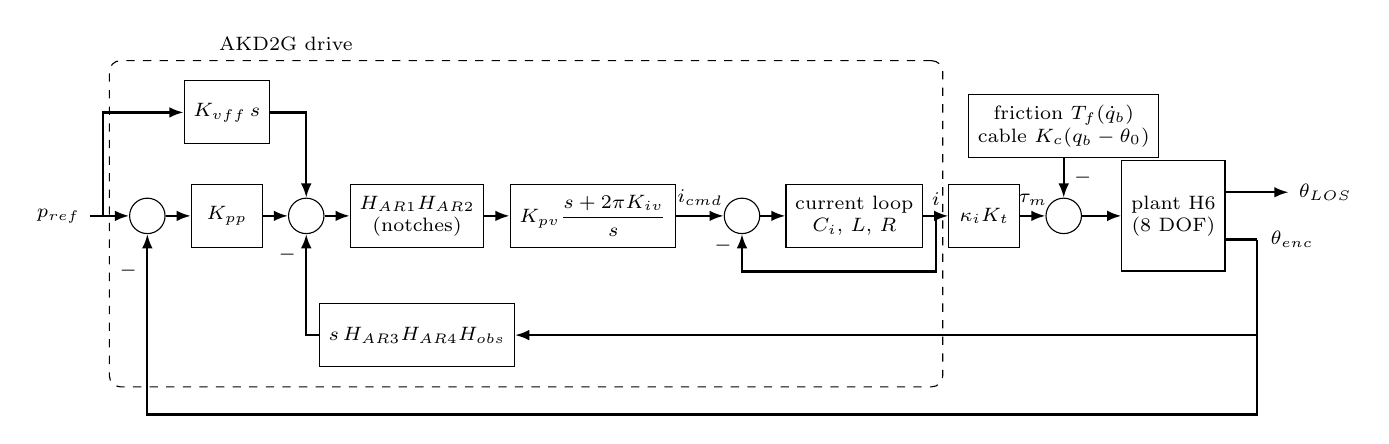
\begin{tikzpicture}[node distance=4mm and 3.2mm]
\node[lab] (in) {$p_{ref}$};
\node[sum, right=5mm of in] (s1) {};
\node[blk, right=of s1] (kpp) {$K_{pp}$};
\node[sum, right=of kpp] (s2) {};
\node[blk, right=of s2] (fwd) {$H_{AR1}H_{AR2}$\\ (notches)};
\node[blk, right=of fwd] (cv) {$K_{pv}\dfrac{s+2\pi K_{iv}}{s}$};
\node[sum, right=6mm of cv] (s3) {};
\node[blk, right=of s3] (ci) {current loop\\ $C_i$, $L$, $R$};
\node[blk, right=of ci] (kt) {$\kappa_iK_t$};
\node[sum, right=of kt] (s4) {};
\node[blk, right=5mm of s4, minimum height=14mm] (pl) {plant H6\\ (8 DOF)};
\node[blk, above=5mm of kpp] (vff) {$K_{vff}\,s$};
\node[blk, below=7mm of fwd] (fb) {$s\,H_{AR3}H_{AR4}H_{obs}$};
\node[blk, above=5mm of s4] (dist) {friction $T_f(\dot q_b)$\\ cable $K_c(q_b-\theta_0)$};
\draw[sig] (in) -- (s1);
\draw[sig] (s1) -- (kpp);
\draw[sig] (kpp) -- (s2);
\draw[sig] (s2) -- (fwd);
\draw[sig] (fwd) -- (cv);
\draw[sig] (cv) -- node[lab, above] {$i_{cmd}$} (s3);
\draw[sig] (s3) -- (ci);
\draw[sig] (ci) -- node[lab, above] {$i$} (kt);
\draw[sig] (kt) -- node[lab, above] {$\tau_m$} (s4);
\draw[sig] (s4) -- (pl);
\draw[sig] (dist) -- node[lab, right] {$-$} (s4);
\draw[sig] ($(in)!0.5!(s1)$) |- (vff);
\draw[sig] (vff) -| (s2);
\draw[sig] ([yshift=3mm]pl.east) -- ++(8mm,0) node[lab, right] {$\theta_{LOS}$};
\coordinate (enc) at ($(pl.east)+(4mm,-3mm)$);
\draw[thick] ([yshift=-3mm]pl.east) -- (enc);
\node[lab, right=0.5mm of enc] {$\theta_{enc}$};
\draw[sig] (enc) |- ($(fb.south)+(0,-6mm)$) -| node[lab, pos=0.9, left] {$-$} (s1);
\draw[sig] (enc |- fb) -- (fb);
\draw[sig] (fb) -| node[lab, pos=0.9, left] {$-$} (s2);
\draw[sig] ($(ci.east)!0.5!(kt.west)$) |- ($(ci.south)+(0,-3mm)$) -| node[lab, pos=0.85, left] {$-$} (s3);
\begin{scope}[on background layer]
\node[grp, fit=(s1)(kpp)(s2)(fwd)(cv)(vff)(fb)(s3)(ci), label={[lab]above left:{AKD2G drive}}] {};
\end{scope}
\end{tikzpicture}
\caption{Current structure, one axis: position P and velocity PI of the drive closed on the encoder ($\theta_{enc}$), velocity feedforward $K_{vff}$ (off in the tests), forward notches on the velocity error, current loop, motor torque $\kappa_iK_ti$ on the plant, which is also loaded by the bearing friction and the cable spring. The pointing error is measured on the line of sight $\theta_{LOS}$ (telescope).}\label{fig:bd_current}
\end{figure}

\subsection{Proposed structure: gyro and reduced-order disturbance observer (Hilkert)}
Hilkert and Pautler~\cite{hilkert2011} add to an inertially stabilised loop a \emph{single-state} disturbance observer: a model of the rigid gimbal driven by the measured motor torque, closed on the gyro rate by one gain $K_o$ (Figure~\ref{fig:bd_obs}):
\begin{equation}
\dot{\hat\omega}=\frac{K_t'\,i_m+\hat T_d}{J'},\qquad \hat T_d=K_o\,(\omega_g-\hat\omega)
\qquad\Longleftrightarrow\qquad
\hat T_d=\underbrace{\frac{K_o/J'}{s+K_o/J'}}_{\text{filter}}\ \underbrace{\bigl(J's\,\omega_g-K_t'\,i_m\bigr)}_{\text{disturbance measurement}} ,\label{eq:obs}
\end{equation}
which is a filtered measurement of the disturbance from Newton's law $T_m+T_d=J\dot\omega$~\cite[eqs.~1--2]{hilkert2011}. The estimate is subtracted from the current command, $i_{ff}=-\hat T_d/K_t'$, so that the motor cancels the disturbance. In the ideal case (rigid gimbal, exact parameters) the observer leaves the command response unchanged and multiplies the disturbance rejection by $s/(s+K_o/J')$~\cite[eqs.~5--6]{hilkert2011}:
\begin{equation}
\frac{\omega_o}{T_d/J}=\frac{1}{s+G_c/J}\cdot\frac{s}{s+K_o/J}.\label{eq:rej}
\end{equation}
For LUCY (Figure~\ref{fig:bd_proposed}) the loops of the drives stay as they are; a rate gyro is added on the telescope and the observer output enters the current command, the point where Hilkert subtracts it when no notch filter sits before the amplifier. As in Hilkert's figure~3, the estimate can pass through a notch on the structural mode.
\begin{figure}[H]\centering
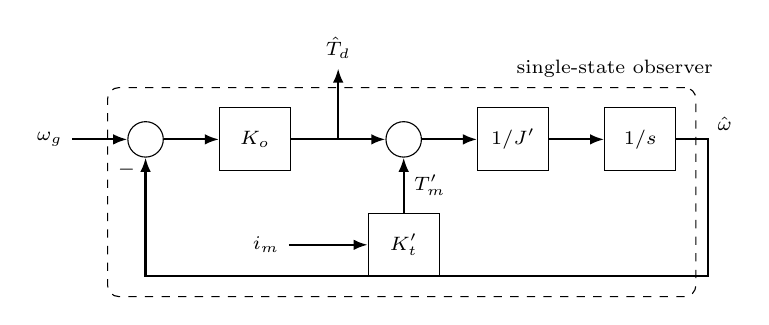
\begin{tikzpicture}[node distance=5mm and 7mm]
\node[lab] (wg) {$\omega_g$};
\node[sum, right=of wg] (e) {};
\node[blk, right=of e] (ko) {$K_o$};
\node[sum, right=12mm of ko] (s) {};
\node[blk, right=of s] (ij) {$1/J'$};
\node[blk, right=of ij] (int) {$1/s$};
\node[blk, below=7mm of s] (ktp) {$K_t'$};
\node[lab, left=10mm of ktp] (im) {$i_m$};
\draw[sig] (wg) -- (e);
\draw[sig] (e) -- (ko);
\draw[sig] (ko) -- coordinate (tdn) (s);
\draw[sig] (tdn) -- ++(0,9mm) node[lab, above] {$\hat T_d$};
\draw[sig] (s) -- (ij);
\draw[sig] (ij) -- (int);
\draw[sig] (int.east) -- ++(4mm,0) |- ($(e.south)+(0,-15mm)$) -- node[lab, pos=0.9, left] {$-$} (e.south);
\node[lab, right=4mm of int, yshift=2mm] {$\hat\omega$};
\draw[sig] (im) -- (ktp);
\draw[sig] (ktp) -- node[lab, right] {$T_m'$} (s);
\begin{scope}[on background layer]
\node[grp, fit=(e)(ko)(s)(ij)(int)(ktp), label={[lab]above right:{single-state observer}}] {};
\end{scope}
\end{tikzpicture}
\caption{Single-state disturbance observer of Hilkert and Pautler~\cite[fig.~3]{hilkert2011}: the model of the rigid axis ($1/J's$) is driven by the motor torque measured through the current, $T_m'=K_t'i_m$, and closed on the gyro rate by the gain $K_o$; the correction is the estimate $\hat T_d$ of the disturbance.}\label{fig:bd_obs}
\end{figure}

\begin{figure}[H]\centering
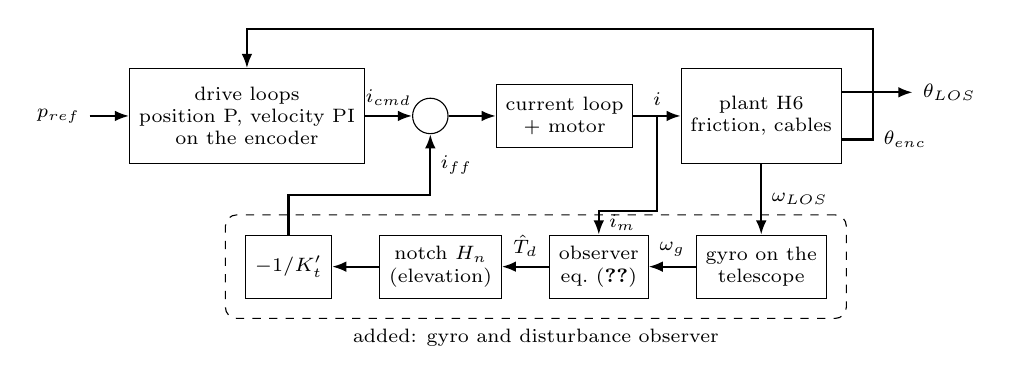
\begin{tikzpicture}[node distance=5mm and 6mm]
\node[lab] (in) {$p_{ref}$};
\node[blk, right=5mm of in, minimum height=12mm] (drv) {drive loops\\ position P, velocity PI\\ on the encoder};
\node[sum, right=of drv] (s3) {};
\node[blk, right=of s3] (ci) {current loop\\ + motor};
\node[blk, right=of ci, minimum height=12mm] (pl) {plant H6\\ friction, cables};
\node[blk, below=9mm of pl] (gyro) {gyro on the\\ telescope};
\node[blk, left=of gyro] (obs) {observer\\ eq.~\eqref{eq:obs}};
\node[blk, left=of obs] (notch) {notch $H_n$\\ (elevation)};
\node[blk, left=of notch] (gain) {$-1/K_t'$};
\draw[sig] (in) -- (drv);
\draw[sig] (drv) -- node[lab, above] {$i_{cmd}$} (s3);
\draw[sig] (s3) -- (ci);
\draw[sig] (ci) -- node[lab, above] {$i$} coordinate[pos=0.5] (im) (pl);
\draw[sig] ([yshift=3mm]pl.east) -- ++(9mm,0) node[lab, right] {$\theta_{LOS}$};
\draw[sig] ([yshift=-3mm]pl.east) -- ++(4mm,0) node[lab, right] {$\theta_{enc}$} |- ($(drv.north)+(0,5mm)$) -- (drv.north);
\draw[sig] (pl) -- node[lab, right] {$\omega_{LOS}$} (gyro);
\draw[sig] (gyro) -- node[lab, above] {$\omega_g$} (obs);
\draw[sig] (im) |- ($(obs.north)+(0,3mm)$) -- node[lab, right] {$i_m$} (obs.north);
\draw[sig] (obs) -- node[lab, above] {$\hat T_d$} (notch);
\draw[sig] (notch) -- (gain);
\draw[sig] (gain.north) -- ++(0,5mm) -| node[lab, pos=0.75, right] {$i_{ff}$} (s3.south);
\begin{scope}[on background layer]
\node[grp, fit=(gyro)(obs)(notch)(gain), label={[lab]below:{added: gyro and disturbance observer}}] {};
\end{scope}
\end{tikzpicture}
\caption{Proposed structure, one axis: the loops of the drive on the encoder are unchanged; a rate gyro on the telescope and the observer of Figure~\ref{fig:bd_obs} give the disturbance estimate, which (through a notch on the structural mode in elevation) is subtracted from the current command.}\label{fig:bd_proposed}
\end{figure}

\subsection{Signal constraints: EtherCAT and the MEMS gyro}
In the real system the observer runs in the EtherCAT master, which exchanges the process data with the drives once per cycle, and reads the gyro over SPI (Figure~\ref{fig:bd_ecat}).
\begin{figure}[H]\centering
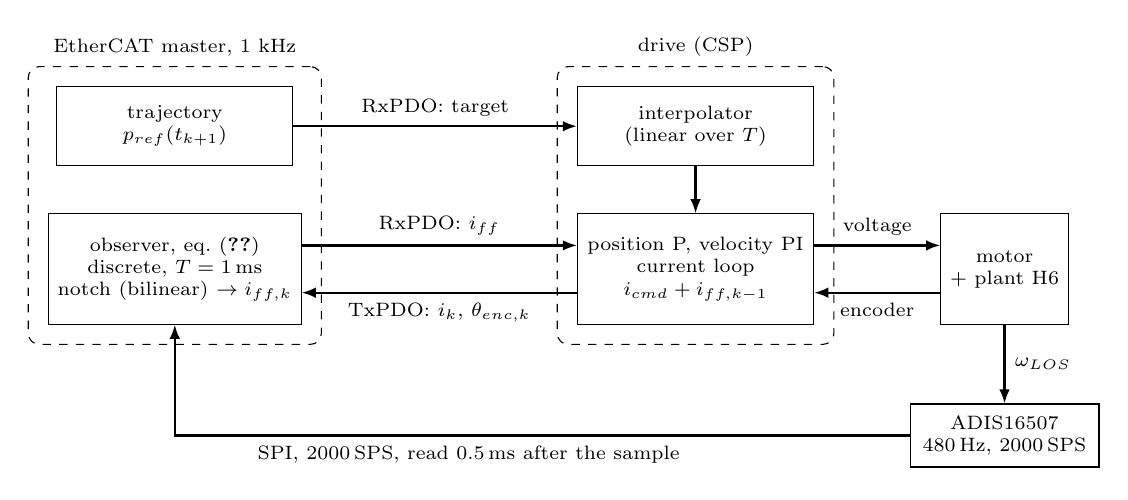
\begin{tikzpicture}[node distance=5mm and 9mm]
\node[blk, minimum width=30mm, minimum height=10mm] (traj) {trajectory\\ $p_{ref}(t_{k+1})$};
\node[blk, below=6mm of traj, minimum width=30mm, minimum height=14mm] (mobs) {observer, eq.~\eqref{eq:obs}\\ discrete, $T=1$\,ms\\ notch (bilinear) $\to i_{ff,k}$};
\node[blk, right=36mm of traj, minimum width=30mm, minimum height=10mm] (interp) {interpolator\\ (linear over $T$)};
\node[blk, below=6mm of interp, minimum width=30mm, minimum height=14mm] (loops) {position P, velocity PI\\ current loop\\ $i_{cmd}+i_{ff,k-1}$};
\node[blk, right=16mm of loops, minimum height=14mm] (pl) {motor\\ + plant H6};
\node[blk, below=10mm of pl, minimum width=24mm] (gyro) {ADIS16507\\ 480\,Hz, 2000\,SPS};
\draw[sig] (traj) -- node[lab, above] {RxPDO: target} (interp);
\draw[sig] (interp) -- (loops);
\draw[sig] ([yshift=3mm]mobs.east) -- node[lab, above] {RxPDO: $i_{ff}$} ([yshift=3mm]loops.west);
\draw[sig] ([yshift=-3mm]loops.west) -- node[lab, below] {TxPDO: $i_k$, $\theta_{enc,k}$} ([yshift=-3mm]mobs.east);
\draw[sig] ([yshift=3mm]loops.east) -- node[lab, above] {voltage} ([yshift=3mm]pl.west);
\draw[sig] ([yshift=-3mm]pl.west) -- node[lab, below] {encoder} ([yshift=-3mm]loops.east);
\draw[sig] (pl) -- node[lab, right] {$\omega_{LOS}$} (gyro);
\draw[sig] (gyro) -| node[lab, pos=0.3, below] {SPI, 2000\,SPS, read 0.5\,ms after the sample} (mobs.south);
\begin{scope}[on background layer]
\node[grp, fit=(traj)(mobs), label={[lab]above:{EtherCAT master, 1 kHz}}] {};
\node[grp, fit=(interp)(loops), label={[lab]above:{drive (CSP)}}] {};
\end{scope}
\end{tikzpicture}
\caption{Sampled-data structure: the master sends each cycle the position target (interpolated by the drive) and the feedforward current computed in the previous cycle (RxPDO), reads the actual current and position (TxPDO) and the gyro over SPI; the drive loops run inside the drive.}\label{fig:bd_ecat}
\end{figure}

%% ===================================================================================================
\section{Implementation step by step}\label{sec:impl}
\subsection{Step 1: closed loop with the identified disturbances}
The closed loop of \texttt{lucy\_cl} (\texttt{ClosedLoop}) received two optional attributes, neutral by default so that the earlier studies and the tests are unchanged:
\begin{itemize}
\item \texttt{torque\_scale}: motor torque $\kappa_iK_ti$ instead of $K_ti$;
\item \texttt{cable\_spring}: torque $-K_c(q_b-\theta_0)$ on the bearing node of each axis, added to the generalised forces.
\end{itemize}
The drives take the I5 gains; the friction elements take the V2 parameters (Table~\ref{tab:model}). The initial state is at rest on the reference, with the friction holding the cable spring.

\subsection{Step 2: reference and commands}
The reference of Section~\ref{sec:task} gives the position command of each axis (relative to the start) and its rate, which is the input of the velocity feedforward. The elevation of the plant is set to the start of the reference, since the inertia of the azimuth depends on it.

\subsection{Step 3: gyro and observer in the continuous loop}
\texttt{GyroObserverLoop} (module \texttt{lucy\_cl.disturbance\_observer}) extends the closed loop with, per axis:
\begin{itemize}
\item \textbf{gyro} on the telescope: elevation $\omega_g=\dot\theta_p$ (telescope node); cross-elevation $\omega_g=\dot\psi_L\cos\theta_p$ (fork node), which the azimuth observer divides by the cosine of the encoder elevation (secant correction);
\item \textbf{observer}~\eqref{eq:obs}, one state $\hat\omega$, with $J'$ the rigid inertia of the axis and $K_t'$ the nominal torque constant. The true torque is $\kappa_iK_ti$ with $\kappa_i=0.96$ and $1.07$: the observer works with a realistic 4--7\,\% error on $K_t$ (Hilkert's sensitivity analysis~\cite[sec.~4]{hilkert2011});
\item \textbf{feedforward} $i_{ff}=-H_n\hat T_d/K_t'$ added to the current command after the velocity PI (the excitation input of the drive model), with $H_n$ an optional chain of biquads.
\end{itemize}

\subsection{Step 4: stability and the notch on the structural mode}\label{sec:stab}
\begin{itemize}
\item \textbf{Method.} The linearised loop (central differences of the time-domain model about rest, the Dahl elements becoming springs $\sigma_0$) is checked through its eigenvalues for each observer bandwidth $f_o=K_o/(2\pi J')$, with the observer on one axis at a time (Table~\ref{tab:stab}).
\item \textbf{Azimuth:} stable up to 80\,Hz.
\item \textbf{Elevation, no notch:} unstable from 8\,Hz. The unstable mode is the first flexible mode of the elevation, about 216\,Hz (telescope against motor): the gyro on the telescope and the motor torque are not collocated, so the observer closes a loop through the structure. This is the instability Hilkert finds when the observer bandwidth approaches the structural resonance~\cite[sec.~5]{hilkert2011}.
\item \textbf{The remedy is Hilkert's:} pass the estimate through a notch at the structural frequency~\cite[fig.~3, fig.~16]{hilkert2011}. With a notch at 210\,Hz ($Q_z=5$, $Q_p=0.5$, $-20$\,dB) the elevation is stable up to 40\,Hz, also with the notch detuned by $\pm10$\,\%.
\end{itemize}
\note{The first elevation mode measured in the October frequency responses is near 95\,Hz, while the model places it at 210\,Hz. In the real system the stability limits are lower and the notch has to be tuned on the measured mode (the elevation drive already has notches at 50 and 96\,Hz on the velocity error).}
\begin{table}[H]\centering\scriptsize\setlength{\tabcolsep}{3pt}
\caption{Stability of the linearised loop with the observer on one axis, against the observer bandwidth: stable, or the frequency of the unstable mode.}\label{tab:stab}
\begin{tabular}{llcccccccc}\toprule
axis & notch & 2\,Hz & 5\,Hz & 7\,Hz & 8\,Hz & 10\,Hz & 20\,Hz & 40\,Hz & 80\,Hz
\\ \midrule
azimuth & no & stable & stable & stable & stable & stable & stable & stable & stable \\
elevation & yes & stable & stable & stable & stable & stable & stable & stable & \textbf{221\,Hz} \\
elevation & no & stable & stable & stable & \textbf{217\,Hz} & \textbf{216\,Hz} & \textbf{215\,Hz} & \textbf{215\,Hz} & \textbf{218\,Hz}
\\ \bottomrule
\end{tabular}\end{table}

\subsection{Step 5: metrics}
\begin{itemize}
\item \textbf{Pointing error}~\cite[eq.~5.23]{attorrese2026}: the angle between the line of sight $\hat n(\psi_L,\theta_p)$ of the telescope and the direction $\hat r$ to the drone,
\begin{equation}
E=\bigl\lVert\hat n(\psi_L,\theta_p)\times\hat r\bigr\rVert,\qquad \hat n=[\cos\theta\cos\psi,\ \cos\theta\sin\psi,\ \sin\theta]^T,
\end{equation}
rms, 95th percentile and maximum over one orbit; also its rms times the distance (miss at the drone).
\item \textbf{Jitter}: rms of the two components of the LOS error (cross-elevation $(\psi_{ref}-\psi_L)\cos\theta_{ref}$, elevation $\theta_{ref}-\theta_p$), high-passed above 1, 10 and 100\,Hz (zero-phase second-order Butterworth). The three values are nested; the rms in a band follows as $\sqrt{J_{f_1}^2-J_{f_2}^2}$.
\end{itemize}

\subsection{Step 6: EtherCAT at 1\,ms}
\texttt{SampledObserverLoop} (module \texttt{lucy\_cl.ethercat}) turns the loop into a sampled-data system with cycle $T=1$\,ms (Figure~\ref{fig:bd_ecat}):
\begin{itemize}
\item \textbf{targets} (RxPDO, cyclic synchronous position): the master sends each cycle the target for the end of the cycle, and the drive interpolates linearly,
\begin{equation}
p(t)=p_{ref}(t_k)+\frac{p_{ref}(t_{k+1})-p_{ref}(t_k)}{T}(t-t_k),\qquad v_{ff}=\frac{p_{ref}(t_{k+1})-p_{ref}(t_k)}{T},\quad t\in[t_k,t_{k+1});
\end{equation}
the alternative of a target held over the cycle (zero-order hold) is also studied;
\item \textbf{actual currents} (TxPDO): sampled at $t_k$ and read by the master;
\item \textbf{observer} in the master, discretised exactly for inputs held over the cycle, with $a=K_o/J'$:
\begin{equation}
\hat T_{d,k}=K_o(\omega_{g,k}-\hat\omega_k),\qquad \hat\omega_{k+1}=e^{-aT}\hat\omega_k+\bigl(1-e^{-aT}\bigr)\Bigl(\omega_{g,k}+\frac{K_t'i_k}{J'a}\Bigr);
\end{equation}
\item \textbf{notch} in the master: bilinear transform prewarped at 210\,Hz (below the 500\,Hz Nyquist frequency);
\item \textbf{feedforward current} (RxPDO): computed from the data of cycle $k$, applied by the drive from $t_{k+1}$ and held for one cycle (one cycle of delay plus the hold).
\end{itemize}
The loops inside the drive (position, velocity, current) stay continuous. Between two cycles the plant, motors, drives and gyro dynamics are integrated by one Radau solver kept across the cycles (step size, Jacobian and factorisation are reused; the derivative is refreshed at each cycle start because the held inputs jump there).

\subsection{Step 7: the MEMS gyro (ADIS16507)}\label{sec:gyro}
\texttt{MemsGyro} (module \texttt{lucy\_cl.gyro}) models one axis of the gyro of an ADIS16507-1, read over SPI (Table~\ref{tab:gyro}):
\begin{equation}
\omega_g(t_k)=\Bigl[H(s)\bigl(\omega+n_w+b\bigr)\Bigr]_{t=\lfloor(t_k-\tau_l)f_{odr}\rfloor/f_{odr}},\qquad H(s)=\frac{\omega_n^2}{s^2+2\zeta\omega_ns+\omega_n^2},
\end{equation}
\begin{itemize}
\item \textbf{dynamics:} second order with the $-3$\,dB bandwidth of the data sheet (480\,Hz, $\zeta=0.707$), states of the continuous model;
\item \textbf{digital output:} registers updated at 2000\,SPS, read by the master $\tau_l=0.5$\,ms after the sample (data ready and SPI burst read); the latency is a first-order Pad\'e delay in the continuous part;
\item \textbf{noise from the Allan deviation}~\cite{ieee952}:
  \begin{itemize}
  \item angle random walk $N=0.13$\,deg/$\sqrt{\mathrm h}$ = \arwSI$\cdot10^{-5}$\,rad/$\sqrt{\mathrm s}$: white rate noise, Allan deviation $N/\sqrt\tau$;
  \item bias instability $B=2.3$\,deg/h: first-order Gauss--Markov bias whose Allan deviation peaks at $B$ at the time of the minimum, $\tau_B\approx1.89T_c$, with standard deviation $B/0.437$;
  \item the data sheet gives neither the time of the minimum (taken as 50\,s) nor a rate random walk (taken as zero). Over one orbit of 31\,s these terms matter little: the observer differentiates the gyro, and the white noise dominates.
  \end{itemize}
\end{itemize}
The noise is generated on a 16\,kHz grid, filtered by the sensor dynamics and read at the cycle times; the same realisation is used in all cases. Check (Figure~\ref{fig:gyro}): the Allan deviation of a one-hour noise record follows the model and the data-sheet points, and the output noise is \gyroNoise\,deg/s rms against 0.068\,deg/s of the data sheet.
\begin{table}[H]\centering\small
\caption{Gyro model: ADIS16507-1, x and y axes~\cite{adis16507}.}\label{tab:gyro}
\begin{tabular}{lll}\toprule
quantity & value & source \\ \midrule
$-3$\,dB bandwidth & 480\,Hz, second order, $\zeta=0.707$ & data sheet (ADIS16507-1/-2, x, y) \\
output data rate & 2000\,SPS & data sheet \\
latency to the master & 0.5\,ms (one output period) & assumption (data ready + SPI burst) \\
angle random walk & 0.13\,deg/$\sqrt{\mathrm h}$ & data sheet (ADIS16507-1, x, y) \\
in-run bias stability & 2.3\,deg/h & data sheet (ADIS16507-1) \\
time of the Allan minimum & 50\,s & assumption \\
rate random walk, turn-on bias & 0 & not modelled \\
output noise, no filtering & 0.068\,deg/s rms (model \gyroNoise) & data sheet \\ \bottomrule
\end{tabular}\end{table}
\begin{figure}[H]\centering
\includegraphics[width=\linewidth]{figures/ecat_gyro_model.pdf}
\caption{Gyro model. Left: Allan deviation [deg/h] against the averaging time [s]: simulated noise (one hour at 2000\,SPS), model terms, data-sheet points. Right: magnitude [dB] and phase [deg] of the second-order dynamics with the latency.}\label{fig:gyro}
\end{figure}

%% ===================================================================================================
\section{Results with the continuous loop and an ideal gyro}\label{sec:cont}
\begin{table}[H]\centering\small
\caption{Continuous loop, ideal gyro: pointing error [mdeg], jitter [$\mu$rad], rms of the LOS error components [mdeg]; one orbit.}\label{tab:cont}
\begin{tabularx}{\linewidth}{Yrrrrrr}\toprule
case & $E$ rms & $E$ max & jitter $>1$\,Hz & jitter $>10$\,Hz & cross-el. rms & elev. rms \\ \midrule
current: loops on the encoders & 124.11 & 183.7 & 99.4 & 1.89 & 123.82 & 8.48 \\
encoders + gyro observer 5 Hz & 117.66 & 182.6 & 30.5 & 2.03 & 117.51 & 6.03 \\
encoders + gyro observer 10 Hz & 117.66 & 182.6 & 7.93 & 0.586 & 117.50 & 6.04 \\
encoders + gyro observer 20 Hz & 117.66 & 182.6 & 4.42 & 0.0101 & 117.51 & 6.04 \\
encoders + gyro observer 40 Hz & 117.67 & 182.6 & 3.54 & 0.00888 & 117.51 & 6.04 \\
current + velocity feedforward & 26.61 & 130.9 & 99.4 & 1.89 & 26.22 & 4.59 \\
current + velocity feedforward + gyro observer 20 Hz & 2.70 & 7.8 & 4.42 & 0.0101 & 2.70 & 0.05 \\
as above, gyro bandwidth 100 Hz & 2.70 & 7.8 & 4.41 & 0.00957 & 2.70 & 0.05 \\
current + velocity feedforward, alternative azimuth friction & 11.79 & 41.7 & 3.61 & 0.00275 & 10.87 & 4.59 \\
current + velocity feedforward + gyro observer 20 Hz, alternative azimuth friction & 1.68 & 3.0 & 0.407 & 0.00132 & 1.68 & 0.05
\\ \bottomrule
\end{tabularx}\end{table}
\begin{itemize}
\item \textbf{Without the velocity feedforward} the pointing error is the following error of the P position loop, $\dot\psi/K_{pp}$, up to \followAz\,mdeg in azimuth. The observer removes the part due to the disturbances (124 to 118\,mdeg) but not this one: as Hilkert shows, in the ideal case the observer leaves the command response unchanged (eq.~\eqref{eq:rej}, \cite[eq.~5]{hilkert2011}).
\item \textbf{With the velocity feedforward} the disturbances dominate and the observer reduces the pointing error from 26.6 to 2.7\,mdeg rms and the jitter above 1\,Hz from 99 to 4.4\,$\mu$rad.
\item \textbf{The residual of 2.7\,mdeg} is the twist of the azimuth shaft between the motor (where the encoder is) and the fork: the friction torque, cancelled by the motor, still passes through it ($1/k_{\psi,2}=4.4$\,mdeg per N\,m). The encoder follows its command at \encAzDob\,mdeg rms while the LOS differs from it by \twist\,mdeg rms; a loop on the encoders cannot see it.
\item \textbf{The disturbance estimate} follows the disturbance of the model (Figure~\ref{fig:dist}); the small offset in elevation is the 7\,\% error of $K_t'$.
\item \textbf{The linearised rejection} (Figure~\ref{fig:rej}, Section~\ref{sec:rejection}) improves below the loop bandwidth by one to two orders of magnitude, as eq.~\eqref{eq:rej} predicts; in azimuth it levels off at the compliance of the shaft.
\end{itemize}
\begin{figure}[H]\centering
\includegraphics[width=0.9\linewidth]{figures/cont_pointing_error.pdf}
\caption{Continuous loop, ideal gyro: pointing error [mdeg, log scale] against time [s], without (top) and with (middle) the velocity feedforward, and with an alternative azimuth friction (bottom).}\label{fig:contpe}
\end{figure}
\begin{figure}[H]\centering
\includegraphics[width=0.9\linewidth]{figures/cont_disturbance_estimate.pdf}
\caption{Disturbance torque on each axis [N\,m] against time [s]: bearing friction plus cable spring of the model, and the observer estimate $\hat T_d$ (20\,Hz).}\label{fig:dist}
\end{figure}

\subsection{Disturbance rejection: definition and reading of the transfer function}\label{sec:rejection}
\paragraph{Definition.} The time-domain model of the closed loop (plant H6, motors, drives and, when present, gyro and observer) is linearised about rest at the start of the reference, by central differences, as $\dot{\mathbf x}=\mathbf A\mathbf x+\mathbf b_d\,T_b$, $\theta_{LOS}=\mathbf c\,\mathbf x$, where:
\begin{itemize}
\item $T_b$ is a torque applied to the \emph{bearing node} of the axis (fork in azimuth, hub in elevation), the node where the friction and the cable spring act;
\item $\mathbf b_d=[\mathbf 0;\ \mathbf M^{-1}(\mathbf q_0)\,\mathbf e_b;\ \mathbf 0]$ puts it into the accelerations of the plant;
\item $\mathbf c$ selects the line-of-sight coordinate ($\psi_L$, $\theta_p$).
\end{itemize}
Figure~\ref{fig:rej} plots the magnitude of
\begin{equation}
G_d(j\omega)=\frac{\theta_{LOS}(j\omega)}{T_b(j\omega)}=\mathbf c\,(j\omega\mathbf I-\mathbf A)^{-1}\mathbf b_d\qquad[\mathrm{rad/(N\,m)}].\label{eq:gd}
\end{equation}

\paragraph{Why ``sliding friction''.} Linearised at rest, the Dahl element of the bearing, $\dot T_f=\sigma_0\bigl(v-|v|\,T_f/g(v)\bigr)$, becomes a spring of stiffness $\sigma_0$ (pre-sliding): it describes micro-motions of a bearing that sticks, not of one that slides. While tracking, the bearing slides and its torque is set by the speed (Coulomb and Stribeck levels): towards the axis it acts as an external torque. The linearisation therefore sets $\sigma_0\to0$, so that the element leaves $\mathbf A$, and the friction becomes the input itself: $T_b=-T_f+T_{cable}$. The cable stiffness (1.7\,N\,m/rad) stays in $\mathbf A$ and is negligible. Any other torque on the bearing (imbalance, wind, cable reaction) enters through the same function.

\paragraph{Meaning.} By superposition:
\begin{itemize}
\item a sinusoidal bearing torque of amplitude $T$ at frequency $f$ moves the LOS by $|G_d(f)|\,T$;
\item a random torque of spectral density $S_T(f)$ gives a LOS spectral density $|G_d|^2S_T$ and a variance $\sigma_\theta^2=\int|G_d|^2S_T\,df$.
\end{itemize}
$|G_d|$ is thus the gain from the disturbance spectrum to the pointing and jitter spectrum: the lower, the better.

\paragraph{Rigid-body model.} Below the first flexible mode, with an ideal current loop, the axis is an inertia $J$ in the loop of the drive:
\begin{equation}
G_d(s)\simeq\frac{1}{Js^2+\kappa_iK_t\,H_{fwd}(s)\,C_v(s)\bigl(C_p(s)+s\,H_{fb}(s)\bigr)}+c_{e\ell},\label{eq:gdrigid}
\end{equation}
with the transfer functions of the drive (Figure~\ref{fig:bd_current}), and $c_{e\ell}$ the static compliance between the encoder and the LOS discussed below. Without filters the controller is a PID on the error, $k_D=K_{pv}$, $k_P=K_{pv}(K_{pp}+\omega_i)$, $k_I=K_{pv}K_{pp}\omega_i$ ($\omega_i=2\pi K_{iv}$), and
\begin{equation}
G_d(s)\simeq\frac{s}{Js^3+\kappa_iK_t\,(k_Ds^2+k_Ps+k_I)} .
\end{equation}
With the observer (rigid axis, exact parameters), Hilkert's eq.~(6)~\cite{hilkert2011} multiplies the rate response, and therefore the position response, by $s/(s+\omega_o)$: $G_{d,obs}(s)\simeq G_d(s)\,s/(s+\omega_o)+c_{e\ell}$. The dashed lines of Figure~\ref{fig:rej} are eq.~\eqref{eq:gdrigid} with the actual filters of the drive; they follow the full model up to the flexible modes.

\paragraph{Asymptotes.}
\begin{itemize}
\item \textbf{Low frequency, current structure:} $|G_d|\simeq\omega/(\kappa_iK_tk_I)$, rising at $+20$\,dB/decade. The velocity integrator rejects a constant torque completely at steady state. With $\kappa_iK_t=\ktkAz$ and \ktkEl\,N\,m/A and $k_I=\kIAz$ and \kIEl\,A/(rad\,s), this gives \lowCurAz\ and \lowCurEl\,$\mu$rad/(N\,m) at 0.1\,Hz in azimuth and elevation, the same as the full model (Table~\ref{tab:rejection}).
\item \textbf{Low frequency, with the observer:} $|G_d|\simeq\omega^2/(\kappa_iK_tk_I\,\omega_o)$, rising at $+40$\,dB/decade and lower by $\omega/\omega_o$. In elevation the ratio to the current structure follows $|s/(s+\omega_o)|$ (Table~\ref{tab:rejection}, second number against third).
\item \textbf{High frequency:} $|G_d|\to1/(J\omega^2)$, $-40$\,dB/decade, the same for all curves. Above the bandwidths of the loop and of the observer no controller acts and the axis responds as a free inertia (\highHundAz\ and \highHundEl\,$\mu$rad/(N\,m) at 100\,Hz). The observer cannot help there, as eq.~\eqref{eq:rej} shows.
\item \textbf{Maximum} at the rigid closed-loop poles:
  \begin{itemize}
  \item azimuth: \peakGAz\,$\mu$rad/(N\,m) at \peakFAz\,Hz (real poles at 0.26, 1.5 and 5.2\,Hz);
  \item elevation: \peakGEl\,$\mu$rad/(N\,m) at \peakFEl\,Hz, where the current gains place a pair of poles with a damping ratio of only 0.29: a torque near 3\,Hz is amplified.
  \end{itemize}
\end{itemize}

\paragraph{Features.}
\begin{itemize}
\item \textbf{Azimuth:}
  \begin{itemize}
  \item the hump at 10--14\,Hz and the steep fall after it come from the forward biquad of the azimuth drive (pole pair at 14\,Hz, $Q=3$, on the velocity error);
  \item the dip at 65\,Hz comes from the forward resonator at 65\,Hz ($+10$\,dB), which raises the loop gain there.
  \end{itemize}
\item \textbf{Elevation:}
  \begin{itemize}
  \item the resonance and antiresonance at 210--230\,Hz are the first flexible mode (telescope against motor) seen at the LOS;
  \item the notches at 50 and 96\,Hz lower the loop gain locally.
  \end{itemize}
\end{itemize}

\paragraph{Compliance floor in azimuth.} A bearing torque balanced by the motor twists the shaft between the motor (which carries the encoder) and the fork (the LOS). With the encoder held by its loop, the LOS moves by $c_{e\ell}=\floorAz\,\mu$rad/(N\,m), computed from the static stiffness of the model ($=1/k_{\psi,2}$).
\begin{itemize}
\item The observer cancels the acceleration of the axis but not this static twist, which the gyro does not see as a rate. At low frequency all its curves therefore tend to $c_{e\ell}$ (67--75\,$\mu$rad/(N\,m) at 0.1\,Hz).
\item The current structure reaches the same floor only near 0.01\,Hz, where $\omega/(\kappa_iK_tk_I)$ falls to $c_{e\ell}$.
\item In elevation the encoder and the LOS lie on the same side of the torque path (hub to motor), so $c_{e\ell}=\floorEl$.
\end{itemize}

\paragraph{Check against the simulations.} At an azimuth reversal the friction swings from about $+1.8$ to $-1.8$\,N\,m in 0.5--1\,s, with content near 1\,Hz.
\begin{itemize}
\item Half the swing times $|G_d(1\,\mathrm{Hz})|$ gives $1.8\times\oneCurAz\,\mu$rad $\approx$ 2.3\,mrad = 131\,mdeg for the current structure, and $1.8\times\oneDobAz\,\mu$rad $\approx$ 13\,mdeg with the observer at 20\,Hz.
\item The time-domain maxima are 131 and 7.8\,mdeg (Table~\ref{tab:ecat}).
\end{itemize}

\paragraph{Validity.}
\begin{itemize}
\item The function is linear and assumes a sliding bearing. Where the bearing sticks (reversals, the elevation at 0.06\,deg/s) the friction is not an external torque but the stiff pre-sliding spring; there only the time-domain simulations hold.
\item The gyro noise is not in $G_d$; it is treated in Section~\ref{sec:focus}.
\end{itemize}
\begin{table}[H]\centering\scriptsize\setlength{\tabcolsep}{3pt}
\caption{$|G_d|$ [$\mu$rad/(N\,m)] at selected frequencies, full linearised model; in brackets: ratio to the current structure; ratio predicted by Hilkert, $|s/(s+\omega_o)|$.}\label{tab:rejection}
\begin{tabular}{llrllll}\toprule
axis & $f$ [Hz] & current & observer 5\,Hz & observer 10\,Hz & observer 20\,Hz & observer 40\,Hz \\ \midrule
azimuth & 0.1 & 580 & 66.9 (0.12; 0.02) & 71.6 (0.12; 0.01) & 74 (0.13; 0.005) & 75.2 (0.13; 0.0025) \\
 & 1 & 1.27e+03 & 293 (0.23; 0.2) & 178 (0.14; 0.1) & 124 (0.098; 0.05) & 101 (0.08; 0.025) \\
 & 3 & 664 & 410 (0.62; 0.51) & 268 (0.4; 0.29) & 181 (0.27; 0.15) & 136 (0.21; 0.075) \\
 & 10 & 218 & 228 (1; 0.89) & 212 (0.97; 0.71) & 179 (0.82; 0.45) & 150 (0.69; 0.24) \\
 & 30 & 13.5 & 12.7 (0.94; 0.99) & 11.7 (0.87; 0.95) & 9.29 (0.69; 0.83) & 5.4 (0.4; 0.6) \\
\midrule
elevation & 0.1 & 343 & 7.17 (0.021; 0.02) & 3.74 (0.011; 0.01) & 2.03 (0.0059; 0.005) & 1.17 (0.0034; 0.0025) \\
 & 1 & 2.56e+03 & 531 (0.21; 0.2) & 281 (0.11; 0.1) & 153 (0.06; 0.05) & 88.6 (0.035; 0.025) \\
 & 3 & 5.62e+03 & 2.93e+03 (0.52; 0.51) & 1.75e+03 (0.31; 0.29) & 1e+03 (0.18; 0.15) & 589 (0.1; 0.075) \\
 & 10 & 315 & 288 (0.92; 0.89) & 232 (0.74; 0.71) & 156 (0.5; 0.45) & 96.9 (0.31; 0.24) \\
 & 30 & 33.1 & 34.1 (1; 0.99) & 34 (1; 0.95) & 31.7 (0.96; 0.83) & 25.4 (0.77; 0.6)
\\ \bottomrule
\end{tabular}\end{table}
\begin{figure}[H]\centering
\includegraphics[width=\linewidth]{figures/rejection_annotated.pdf}
\caption[Disturbance rejection, bearing torque to line of sight]{Disturbance rejection $|G_d|$, eq.~\eqref{eq:gd}: LOS angle per N\,m of torque on the bearing [$\mu$rad/(N\,m)] against frequency [Hz]. Solid lines: full linearised loops (sliding friction), current structure and observer bandwidths. Dashed lines: rigid-body model, eq.~\eqref{eq:gdrigid}, with the filters of the drive, for the current structure and the observer at 20\,Hz. Dotted lines: asymptotes $\omega/(\kappa_iK_tk_I)$, $\omega^2/(\kappa_iK_tk_I\omega_o)$ and $1/(J\omega^2)$. Dash-dotted line: compliance floor between the encoder and the LOS (azimuth).}\label{fig:rej}
\end{figure}

%% ===================================================================================================
\section{Focus: pointing error and jitter, current structure against the observer with the noisy gyro}\label{sec:focus}
Constraints of Section~\ref{sec:impl} (EtherCAT 1\,ms, ADIS16507 read over SPI), velocity feedforward on, observer at 20\,Hz with the notch in elevation; the observer with a noise-free gyro (same EtherCAT and gyro dynamics) separates the effect of the noise.
\begin{table}[H]\centering\small
\caption{Pointing error [mdeg], miss at the drone [mm] and jitter by band [$\mu$rad]; one orbit.}\label{tab:focus}
\begin{tabular}{lrrrrrrrr}\toprule
& \multicolumn{4}{c}{pointing error} & \multicolumn{4}{c}{jitter [$\mu$rad]} \\ \cmidrule(lr){2-5}\cmidrule(lr){6-9}
case & rms & 95\,\% & max & miss [mm] & $>1$\,Hz & 1--10\,Hz & 10--100\,Hz & $>100$\,Hz \\ \midrule
current (encoders) & 26.62 & 55.44 & 131.0 & 46.4 & 98.9 & 98.8 & 1.88 & $4.63\cdot10^{-4}$ \\
observer 20\,Hz, ideal gyro & 2.70 & 6.99 & 7.7 & 4.7 & 5.04 & 5.04 & 0.0112 & $3.14\cdot10^{-6}$ \\
observer 20\,Hz, ADIS16507 & 2.72 & 6.92 & 8.0 & 4.8 & 9.65 & 9.29 & 2.61 & 0.142
\\ \bottomrule
\end{tabular}\end{table}
\begin{table}[H]\centering\small
\caption{The same in degrees.}\label{tab:focusdeg}
\begin{tabular}{lrrrrrr}\toprule
case & $E$ rms [deg] & $E$ max [deg] & jitter $>1$\,Hz & 1--10\,Hz & 10--100\,Hz & $>100$\,Hz [deg] \\ \midrule
current (encoders) & 0.027 & 0.13 & $5.7\cdot10^{-3}$ & $5.7\cdot10^{-3}$ & $1.1\cdot10^{-4}$ & $2.7\cdot10^{-8}$ \\
observer 20\,Hz, ideal gyro & $2.7\cdot10^{-3}$ & $7.7\cdot10^{-3}$ & $2.9\cdot10^{-4}$ & $2.9\cdot10^{-4}$ & $6.4\cdot10^{-7}$ & $1.8\cdot10^{-10}$ \\
observer 20\,Hz, ADIS16507 & $2.7\cdot10^{-3}$ & $8.0\cdot10^{-3}$ & $5.5\cdot10^{-4}$ & $5.3\cdot10^{-4}$ & $1.5\cdot10^{-4}$ & $8.1\cdot10^{-6}$
\\ \bottomrule
\end{tabular}\end{table}

\subsection{Pointing error}
\begin{itemize}
\item The observer lowers the pointing error from \ErmsCur\ to \ErmsDob\ mdeg rms (\EratioRms\ times) and from \EmaxCur\ to \EmaxDob\ mdeg at the peak (\EratioMax\ times); at 100\,m this is a miss of a few millimetres. The peaks of the current structure are the velocity reversals of the azimuth, where the friction passes through its Stribeck peak (Figure~\ref{fig:ecatpe}).
\item The gyro noise does not change the pointing error (\ErmsIdeal\ against \ErmsDob\ mdeg): it is a zero-mean, mostly high-frequency error, while the pointing error is dominated by the shaft twist and by the low-frequency residual of the friction.
\item EtherCAT at 1\,ms is invisible at this level: with the targets held instead of interpolated the pointing error is \ErmsZoh\ mdeg with the observer and \ErmsCurZoh\ mdeg without.
\item All cases are well inside the threshold of 0.2\,deg recalled by Attorrese.
\end{itemize}
\begin{figure}[H]\centering
\includegraphics[width=0.9\linewidth]{figures/ecat_pointing_error.pdf}
\caption{EtherCAT and ADIS16507: pointing error [mdeg, log scale] against time [s], current structure and observer, without (top) and with (bottom) the velocity feedforward; dashed: the observer in the continuous loop with an ideal gyro.}\label{fig:ecatpe}
\end{figure}

\subsection{Jitter}
Figure~\ref{fig:bands} splits the jitter by band and Figure~\ref{fig:cum} gives the rms of the LOS error above each frequency.
\begin{itemize}
\item \textbf{1--10\,Hz, the band that dominates the jitter:} \BandOneTenCur\ $\mu$rad with the current structure, \BandOneTenDob\ $\mu$rad with the observer. Here sit the friction transients at the azimuth reversals, and here the observer acts, below its bandwidth. The jitter above 1\,Hz therefore falls \JoneRatio\ times, from \JoneCur\ to \JoneDob\ $\mu$rad.
\item \textbf{The gyro noise} adds about \NoiseJone\ $\mu$rad to the jitter above 1\,Hz (\JoneIdeal\ $\mu$rad with an ideal gyro). Below its bandwidth the observer makes the LOS follow the inertial rate measured by the gyro, and therefore also the integral of its white noise (angle random walk) between the bandwidth of the position loop ($f_1\approx1$\,Hz) and that of the observer ($f_o$):
\begin{equation}
\sigma_{LOS}\approx\frac{N}{2\pi}\sqrt{\frac1{f_1}-\frac1{f_o}}\approx\noiseFloor\ \mu\text{rad},
\end{equation}
consistent with the simulation. This floor scales with the angle random walk of the gyro.
\item \textbf{10--100\,Hz:} \BandTenHunDob\ $\mu$rad with the observer against \BandTenHunCur\ $\mu$rad, slightly worse. With an ideal gyro this band would almost vanish (\JtenIdeal\ $\mu$rad above 10\,Hz); with the ADIS16507 it is the gyro noise.
\item \textbf{Above 100\,Hz:} \JhunDob\ $\mu$rad against \JhunCur\ $\mu$rad, more than two orders of magnitude higher but negligible in absolute terms (less than 0.1\,\% of the total). The current structure is that clean only because the model has no other noise source (encoder quantisation and noise, current measurement, PWM): the comparison in this band is not a fair one.
\item \textbf{Noise-equivalent current} (Figure~\ref{fig:iff}): the feedforward current of the azimuth carries about \IffNoise\,A rms of noise (\IffAz\,A rms against \IffAzIdeal\,A with an ideal gyro), flat between the observer bandwidth and the gyro bandwidth, as Hilkert's eq.~(10) predicts~\cite{hilkert2011}. It heats the motor and uses part of the current margin, but does not reach the LOS, filtered by the inertia.
\end{itemize}
\begin{figure}[H]\centering
\includegraphics[width=0.85\linewidth]{figures/jitter_bands.pdf}
\caption{Jitter by frequency band [$\mu$rad, log scale]: rms of the LOS error in 1--10\,Hz, 10--100\,Hz, above 100\,Hz and in total above 1\,Hz; current structure, observer with an ideal gyro, observer with the ADIS16507.}\label{fig:bands}
\end{figure}
\begin{figure}[H]\centering
\includegraphics[width=\linewidth]{figures/cumulative_jitter.pdf}
\caption{Rms of the LOS error above each frequency [$\mu$rad] against frequency [Hz], cross-elevation and elevation: where the jitter comes from.}\label{fig:cum}
\end{figure}
\begin{figure}[H]\centering
\includegraphics[width=\linewidth]{figures/ecat_components_ff.pdf}
\caption{EtherCAT and ADIS16507, velocity feedforward: LOS error components [mdeg] against time [s] (top), error above 1\,Hz [$\mu$rad] (middle) and amplitude spectral density [$\mu$rad/$\sqrt{\mathrm{Hz}}$] (bottom); current structure, observer with the noisy gyro, observer with an ideal gyro.}\label{fig:ecatcomp}
\end{figure}
\begin{figure}[H]\centering
\includegraphics[width=\linewidth]{figures/ecat_feedforward_current.pdf}
\caption{Feedforward current of the observer [A] against time [s] (top) and its amplitude spectral density [A/$\sqrt{\mathrm{Hz}}$] (bottom), noisy and ideal gyro.}\label{fig:iff}
\end{figure}

\subsection{Required motor torque}\label{sec:torque}
Figure~\ref{fig:torque} and Table~\ref{tab:torque} give the motor torque $\tau_m=\kappa_iK_t\,i$ of the three cases of Table~\ref{tab:focus}.
\begin{itemize}
\item \textbf{What the torque is made of.}
  \begin{itemize}
  \item The inertial part of the reference is negligible: $J\ddot\theta_{ref}$ is at most \tauInertiaAz\,mN\,m in azimuth and \tauInertiaEl\,mN\,m in elevation.
  \item The cable spring is almost constant (\cableAz\ and \cableEl\,N\,m).
  \item The required torque is therefore the friction torque. In azimuth it is about $\pm0.2$--0.4\,N\,m while sliding, with peaks of $\pm\tauPkCurAz$\,N\,m at the velocity reversals (Stribeck peak $T_s=1.84$\,N\,m). In elevation it is close to the break-away level $T_s=0.46$\,N\,m plus the cable spring, with the sign set by the direction of the slow motion.
  \end{itemize}
\item \textbf{Current structure against the observer with an ideal gyro.} The rms and peak torques are the same (\tauRmsCurAz\ and \tauRmsIdealAz\,N\,m rms in azimuth, \tauRmsCurEl\ and \tauRmsIdealEl\ in elevation): the observer does not ask for more torque, it delivers the same torque \emph{earlier}.
  \begin{itemize}
  \item At the azimuth reversal (middle of Figure~\ref{fig:torque}) the observer reverses the torque as soon as the friction does.
  \item The current structure keeps it for about another second, while its velocity integrator winds up through the error. That delay is the 131\,mdeg peak of the pointing error.
  \item In elevation the same holds at the reversal of the slow motion.
  \end{itemize}
\item \textbf{With the ADIS16507:}
  \begin{itemize}
  \item the torque carries the gyro noise, differentiated by the observer: \tauHiDobAz\,N\,m rms above 10\,Hz in azimuth and \tauHiDobEl\ in elevation, with a flat spectrum from the observer bandwidth to the gyro bandwidth (Figure~\ref{fig:torque}, bottom; the elevation notch at 210\,Hz is visible);
  \item the azimuth peak grows to \tauPkDobAz\,N\,m (40\,\% of the peak torque of the motor, \tPeak\,N\,m);
  \item the rms grows by about 10\,\% and the copper losses, proportional to $i^2$, by about 20\,\%.
  \end{itemize}
  All values stay well inside the limits of the motor (continuous stall torque \tCont\,N\,m).
\item \textbf{Elevation, lower low-frequency torque with the noisy gyro} (\tauLoDobEl\ against \tauLoIdealEl\,N\,m). The noise current acts on the bearing as a \emph{dither}~\cite[sec.~11.2.2]{gawronski2008}: the Dahl element, cycled by the high-frequency torque, carries a lower mean friction (mean $|T_f|$ \fricDobEl\ against \fricIdealEl\,N\,m). This is a property of the friction model; a real bearing behaves qualitatively the same, but the size of the effect should not be taken at face value.
\end{itemize}
\begin{table}[H]\centering\small
\caption{Motor torque $\kappa_iK_ti$ over one orbit, EtherCAT and velocity feedforward: rms and peak [N\,m], rms of its parts below and above 10\,Hz [N\,m], rms against the continuous stall torque and peak against the peak torque of the motor [\%].}\label{tab:torque}
\begin{tabular}{llrrrrrr}\toprule
axis & case & rms & peak & rms $<10$\,Hz & rms $>10$\,Hz & rms/$T_{cont}$ & peak/$T_{peak}$ \\ \midrule
azimuth & current (encoders) & 0.646 & 1.84 & 0.645 & 0.012 & 30 & 27 \\
 & observer 20 Hz, ideal gyro & 0.633 & 1.84 & 0.633 & 0.000 & 29 & 27 \\
 & observer 20 Hz, ADIS16507 & 0.709 & 2.69 & 0.627 & 0.330 & 33 & 40 \\
elevation & current (encoders) & 0.461 & 0.62 & 0.461 & 0.000 & 21 & 9 \\
 & observer 20 Hz, ideal gyro & 0.460 & 0.62 & 0.460 & 0.000 & 21 & 9 \\
 & observer 20 Hz, ADIS16507 & 0.374 & 0.97 & 0.357 & 0.109 & 17 & 14
\\ \bottomrule
\end{tabular}\end{table}
\begin{figure}[H]\centering
\includegraphics[width=\linewidth]{figures/torque_profile.pdf}
\caption{Motor torque [N\,m] of the current structure and of the observer at 20\,Hz with an ideal and with the ADIS16507 gyro, EtherCAT and velocity feedforward: over one orbit against time [s] (top), around the first velocity reversal of each axis (\revAz\ and \revEl\,s, middle), and amplitude spectral density [N\,m/$\sqrt{\mathrm{Hz}}$] against frequency [Hz] (bottom).}\label{fig:torque}
\end{figure}

\subsection{Choice of the observer bandwidth}
Figure~\ref{fig:sweep} repeats the comparison for observer bandwidths of 5--40\,Hz, with the noisy and the ideal gyro.
\begin{itemize}
\item The jitter above 1\,Hz is \JsweepFive, \JsweepTen, \JsweepTwenty\ and \JsweepForty\ $\mu$rad at 5, 10, 20 and 40\,Hz: below 20\,Hz the friction transients are not rejected enough, above it the gyro noise grows faster than the rejection. 20\,Hz is the best of the four.
\item The jitter above 10 and 100\,Hz and the noise current grow with the bandwidth, as Hilkert's figures~10--13 show~\cite{hilkert2011}.
\item The pointing error does not improve beyond 10--20\,Hz.
\end{itemize}
\begin{figure}[H]\centering
\includegraphics[width=\linewidth]{figures/ecat_observer_sweep.pdf}
\caption{EtherCAT, velocity feedforward: pointing error rms [mdeg] and jitter above 1, 10 and 100\,Hz [$\mu$rad] against the observer bandwidth [Hz], noisy and ideal gyro, and the current structure.}\label{fig:sweep}
\end{figure}

\subsection{Overall table}
\begin{table}[H]\centering\scriptsize
\caption{EtherCAT and ADIS16507, all cases: pointing error [mdeg], jitter [$\mu$rad], feedforward current rms azimuth / elevation [A]; one orbit.}\label{tab:ecat}
\begin{tabularx}{\linewidth}{Yrrrrrr}\toprule
case & $E$ rms & $E$ max & jitter $>1$\,Hz & $>10$\,Hz & $>100$\,Hz & $i_{ff}$ rms \\ \midrule
current (encoders) & 124.11 & 183.7 & 98.9 & 1.88 & 0.000463 & 0.00 / 0.00 \\
current + gyro observer 20 Hz & 117.66 & 183.0 & 9.66 & 2.63 & 0.142 & 2.86 / 1.35 \\
current + velocity FF & 26.62 & 131.0 & 98.9 & 1.88 & 0.000463 & 0.00 / 0.00 \\
current + velocity FF + gyro observer 5 Hz & 3.90 & 15.2 & 42.5 & 2.92 & 0.0344 & 2.47 / 1.63 \\
current + velocity FF + gyro observer 10 Hz & 2.93 & 10.1 & 18.4 & 2.41 & 0.0695 & 2.62 / 1.55 \\
current + velocity FF + gyro observer 20 Hz & 2.72 & 8.0 & 9.65 & 2.61 & 0.142 & 2.86 / 1.35 \\
current + velocity FF + gyro observer 40 Hz & 2.78 & 8.5 & 10.3 & 3.2 & 0.29 & 3.72 / 1.21 \\
as dob5\_ff, gyro without noise & 3.63 & 15.0 & 33.9 & 2.25 & 0.000407 & 2.52 / 1.67 \\
as dob10\_ff, gyro without noise & 2.84 & 9.8 & 12 & 1.15 & 0.000164 & 2.55 / 1.66 \\
as dob20\_ff, gyro without noise & 2.70 & 7.7 & 5.04 & 0.0112 & 3.14e-06 & 2.55 / 1.66 \\
as dob40\_ff, gyro without noise & 2.70 & 7.8 & 4.08 & 0.00822 & 2.46e-06 & 2.55 / 1.66 \\
current + velocity FF, targets held (zoh) & 26.70 & 131.2 & 98.9 & 1.88 & 0.000463 & 0.00 / 0.00 \\
current + velocity FF + gyro observer 20 Hz, targets held (zoh) & 2.90 & 8.0 & 9.65 & 2.61 & 0.142 & 2.86 / 1.35
\\ \bottomrule
\end{tabularx}\end{table}

%% ===================================================================================================
\section{Limits and next steps}\label{sec:next}
\paragraph{Limits.}
\begin{itemize}
\item The structural mode of the elevation in the model (210\,Hz) is not the measured one (about 95\,Hz): the stability limits and the notch must be revised on the real mode.
\item The azimuth Stribeck peak ($T_s/T_c=7.9$) is the least determined parameter of the identification. With the alternative friction of the identification ($T_s/T_c=2.66$) the absolute values change, but the observer still gains 7--9 times (continuous study).
\item Only the gyro is noisy: encoder quantisation and noise, current measurement noise and PWM are not modelled, so the high-frequency jitter of the current structure is optimistic.
\item The drive loops are continuous; the data-sheet values of the gyro without a time of the Allan minimum and a rate random walk are completed by assumptions.
\end{itemize}
\paragraph{Next steps.}
\begin{itemize}
\item A low pass on the observer output (or on both its inputs, not on the gyro alone, which would create a false disturbance during the accelerations) at 3--5 times the observer bandwidth: it halves the noise current and lowers the jitter above 100\,Hz, but not the dominant 1--10\,Hz part.
\item A gyro with a lower angle random walk (the noise floor scales with it), or a lower observer bandwidth where the friction allows it.
\item The twist of the azimuth shaft (2.7\,mdeg) needs the LOS position: a loop on the integrated gyro or on an optical sensor, or the predicted twist $\hat T_d/k_{\psi,2}$ added to the position command.
\item Encoder and current noise in the model, for a fair comparison of the high-frequency jitter.
\end{itemize}

\begin{thebibliography}{9}
\bibitem{hilkert2011} J.~M.~Hilkert, B.~Pautler, ``A reduced-order disturbance observer applied to inertially stabilized line-of-sight control'', \emph{Proc. SPIE} 8052, Acquisition, Tracking, Pointing, and Laser Systems Technologies XXV, 80520H, 2011. doi:10.1117/12.884123.
\bibitem{hilkert2008} J.~M.~Hilkert, ``Inertially stabilized platform technology: concepts and principles'', \emph{IEEE Control Systems Magazine}, 28(1):26--46, 2008.
\bibitem{gawronski2008} W.~Gawronski, \emph{Modeling and Control of Antennas and Telescopes}, Springer, New York, 2008.
\bibitem{attorrese2026} L.~Attorrese, \emph{Application of distributed MPC algorithms to a pointer-drone system}, master's thesis in Automation and Control Engineering (advisor M.~Farina), Politecnico di Milano, 2026; sections 5.3 and 6.2.
\bibitem{adis16507} Analog Devices, \emph{ADIS16507 Precision, Miniature MEMS IMU}, data sheet Rev.~A.
\bibitem{ieee952} IEEE Std 952-1997, \emph{IEEE Standard Specification Format Guide and Test Procedure for Single-Axis Interferometric Fiber Optic Gyros} (Annex C: Allan variance noise terms).
\end{thebibliography}
\end{document}
